% =====================================================================
%  ICDEC 2026  ---  Springer Lecture Notes in Networks and Systems (LNNS)
%  Class: llncs (Springer Proceedings LaTeX2e). Available in TeX Live and
%  on Overleaf, so this project compiles on upload with no extra files.
%  Length target: 10 pages (min 8, max 12) including figures and references.
% =====================================================================
\documentclass[runningheads]{llncs}

\usepackage{graphicx}
\usepackage{booktabs}
\usepackage{amsmath}
\usepackage{amssymb}
\usepackage[T1]{fontenc}
\usepackage{hyperref}
\renewcommand\UrlFont{\color{blue}\rmfamily}

\usepackage{placeins}   % \FloatBarrier

% Float control. With [t]-only placement LaTeX can defer a float past the end of
% the document and drop it ("Float(s) lost"). These settings let floats sit on a
% text page and keep them near the text that cites them.
\renewcommand{\topfraction}{0.90}
\renewcommand{\bottomfraction}{0.70}
\renewcommand{\textfraction}{0.10}
\renewcommand{\floatpagefraction}{0.75}
\setcounter{topnumber}{3}
\setcounter{bottomnumber}{2}
\setcounter{totalnumber}{5}

\graphicspath{{figures/}}

\begin{document}

\title{When Does a Second Variance Factor Pay? Pre-Specified Held-Out
Evidence from Five Cryptocurrency Option Markets}

\titlerunning{When Does a Second Variance Factor Pay?}

\author{%
Dhruva Ambhaikar\inst{1}\orcidID{0009-0008-1823-7221} \and
Dhurva Bamb\inst{1}\orcidID{0009-0003-5413-1890} \and
Viraj Choudhary\inst{1}\orcidID{0009-0005-9782-8246} \and
Kapil Rathor\inst{1}\orcidID{0000-0002-7630-3118} \and
Anagha Raich\inst{1}}

\authorrunning{D. Ambhaikar et al.}

\institute{Department of Artificial Intelligence,\\
Mukesh Patel School of Technology Management and Engineering,\\
SVKM's NMIMS, Mumbai, India}

\maketitle

\begin{abstract}
Two-factor stochastic volatility models are widely believed to price options
better than one-factor models, because they can represent a fast and a slow
source of variance at the same time. That belief is rarely tested in a way that
could have falsified it. We report a comparison of Black--Scholes, the
Heston model and the Double-Heston model under a protocol frozen and hashed
before any option data was downloaded, on 16,186 option quotes (5,214 of them
held out under the primary design) drawn from five cryptocurrency markets on the Deribit venue: Bitcoin,
Ether, Solana, XRP and Hyperliquid. Every evaluation date was selected from
volatility-index or spot data before any option data was downloaded, every
model was calibrated separately on each date, and accuracy was measured only on
quotes and expiries withheld from calibration. Significance required a
one-sided Wilcoxon signed-rank test \emph{and} a cluster-bootstrap lower bound
above zero, so that neither test alone could produce a result. The
Double-Heston model beat Black--Scholes on every asset, reducing median
implied-volatility error from 8.13 to 1.86 volatility points on Bitcoin shock
dates. Against the one-factor Heston model the picture differs sharply: Double
Heston won decisively on Bitcoin and Ether and failed to win on Solana, XRP and
Hyperliquid. The two markets where it won are the two that quote six to seven
expiries per day; the three where it did not quote about four. We argue that
the second variance factor pays only when the surface contains enough distinct
maturities to identify two mean-reversion speeds, and that reporting only
favourable markets conceals this boundary.

\keywords{Stochastic volatility \and Double Heston \and Option pricing \and
Cryptocurrency derivatives \and Model identifiability \and Held-out evaluation}
\end{abstract}

% =====================================================================
\section{Introduction}

Anyone pricing options must decide how much structure to buy. Black--Scholes
assumes one constant volatility and is wrong in a way every practitioner can
see: implied volatility varies with both strike and maturity. Heston replaces
that constant with a mean-reverting variance process and captures much of the
variation. The natural next step, taken by the Double-Heston model, is to add
a second variance process on a different time scale: short-dated options
respond to volatility that mean-reverts quickly and long-dated options to a
slower component, and one process cannot be fast and slow at once.

The argument is appealing, but the extra factor is not free. It doubles the
variance parameters from five to ten, and those parameters must be recovered
from a finite set of quoted prices. If the quoted surface does not contain
enough distinct maturities, two mean-reversion speeds cannot be told apart, and
the additional flexibility buys nothing while making calibration harder.
Whether the trade is worthwhile is therefore an empirical question, and it is a
question about the \emph{data} as much as about the model.

Most published comparisons answer it on one market, usually a major equity
index, and report a favourable result; such a design cannot reveal where the
advantage stops. This study is built to locate that boundary rather than to
demonstrate the advantage, testing the same three models on five
cryptocurrency markets that differ sharply in how many expiries they quote,
with every choice that could bias the outcome fixed before any option price
was observed.

Our contributions are:

\begin{enumerate}
\item A pre-specified, five-market comparison of Black--Scholes, Heston and
Double Heston in which the evaluation dates were selected from volatility or
spot data before any option data was fetched, and the success criterion was
fixed in advance.
\item Evidence that the Double-Heston advantage over Black--Scholes is large
and universal across these markets, while its advantage over one-factor Heston
is \emph{conditional} and appears only where the surface quotes roughly six or
more expiries per day.
\item An identifiability explanation for that boundary, supported both by the
negative results and by the contrast with a secondary design in which no
separation of time scales is required and the two-factor model then wins
almost everywhere.
\item Full disclosure of a defect found in our own baseline implementation,
the frozen correction, and both sets of results.
\end{enumerate}

We do not claim that Double Heston is the best available model, that these
results transfer to equity or foreign-exchange markets, or that they imply a
trading strategy. We claim something narrower: the value of a second variance
factor depends on whether the market supplies enough maturities to estimate it.

% =====================================================================
\section{Related Work}

Classical option valuation rests on Black--Scholes \cite{black1973} and
Merton \cite{merton1973}, with Black's forward formulation \cite{black1976}
matching the contract conventions used here; the observed variation of implied
volatility across strikes and maturities motivates richer models
\cite{gatheral2006}. Heston \cite{heston1993} made stochastic volatility
tractable. Bakshi, Cao and Chen \cite{bakshi1997} found that stochastic
volatility, stochastic rates and jumps have different implications for pricing
than for hedging; Bates \cite{bates2000} studied post-crash S\&P~500 futures
options and Duffie, Pan and Singleton \cite{duffie2000} developed transform
methods for affine jump-diffusions. Most directly, Christoffersen, Heston and
Jacobs \cite{chj2009} showed that multiple variance factors capture both the
shape and the term structure of equity-index smiles. That motivates testing a
second factor; it does not establish that the benefit carries over to
cryptocurrency markets.

Making such a test meaningful requires accurate, stable valuation: FFT
\cite{carr1999} and Fourier-cosine \cite{fang2008} methods, careful handling of
complex logarithms \cite{lord2010}, efficient calibration \cite{cui2017}, and
the square-root boundary analysed by Feller \cite{feller1951}, whose constraint
we treat as a separate modelling choice.

In cryptocurrency, Madan, Reyners and Schoutens \cite{madan2019} calibrated
several models to Bitcoin options, Hou et al.\ \cite{hou2020} added stochastic
volatility with correlated jumps, and Alexander and Imeraj built Deribit
implied-volatility indices \cite{alexander2021} and evaluated smile-adjusted
delta hedging \cite{alexander2023}. None asks how the held-out benefit of a
second variance factor varies across markets with different maturity coverage,
which is the question here.

We therefore compare a term-structure Black baseline, one-factor and two-factor
Heston on predefined partitions, including withheld expiries. Because dates
cluster into episodes, comparisons are made at the cluster level using the
Wilcoxon signed-rank procedure \cite{wilcoxon1945} with bootstrap
\cite{efron1979} and clustered-resampling \cite{cameron2008} inference. Fixing
the protocol in advance follows the rationale for preregistered research
decisions \cite{nosek2018}; Section~4 states the configuration, the freeze
record and the manifests.

\section{Models and Numerical Method}

All models are priced in a forward-normalised, undiscounted convention. With
$F$ the forward price at the option's expiry, $K$ the strike,
$x=\log(F/K)$ the log-forward moneyness and $\tau$ the time to maturity in
years, we work with the normalised call value $c = C/F$. This removes the
discount factor and the level of the underlying from the comparison and matches
how the venue quotes its contracts.

\subsection{Black--Scholes with a Term Structure}

The constant-volatility model is given one volatility \emph{per expiry} rather
than one for the whole surface. This is a deliberately generous baseline: it
absorbs the entire maturity dimension of the smile and leaves only the strike
dimension unexplained. A quote in a calibrated expiry is priced with that
expiry's volatility; a quote in a withheld expiry is priced by interpolating
total variance linearly between neighbouring calibrated expiries, with a flat
extension beyond them.

\subsection{Heston and Double Heston}

The one-factor model is
\begin{align}
\frac{dF}{F} &= \sqrt{v}\,dW_1, \\
dv &= \kappa(\theta - v)\,dt + \sigma\sqrt{v}\,dW_2,
\qquad \mathrm{corr}(dW_1,dW_2)=\rho,
\end{align}
with five parameters $(\kappa,\theta,\sigma,\rho,v_0)$. Here $\kappa$ is the
speed at which variance returns to its long-run level $\theta$, $\sigma$ is the
volatility of variance, $\rho$ couples spot and variance shocks and produces
the skew, and $v_0$ is the variance today.

The Double-Heston model drives the same underlying with two independent
square-root processes,
\begin{align}
\frac{dF}{F} &= \sqrt{v_1}\,dW_1 + \sqrt{v_2}\,dW_3, \\
dv_i &= \kappa_i(\theta_i - v_i)\,dt + \sigma_i\sqrt{v_i}\,dW_{2i},
\qquad i = 1,2,
\end{align}
with $\mathrm{corr}(dW_1,dW_2)=\rho_1$ and $\mathrm{corr}(dW_3,dW_4)=\rho_2$,
the two factors being mutually independent. This gives ten parameters,
$(\kappa_i,\theta_i,\sigma_i,\rho_i,v_{i,0})$ for $i=1,2$.
The intended division of labour is that one factor
reverts quickly and governs short-dated options while the other reverts slowly
and governs long-dated ones. Because the factors are independent, the
characteristic function of the log-forward is the product of the two
single-factor characteristic functions, so pricing costs roughly twice that of
one-factor Heston.

\subsection{Numerical Reference}

Prices are obtained by Gauss--Laguerre inversion of the characteristic function
using a parameterisation that avoids branch-cut discontinuities
\cite{lord2010}. A 128-node result is checked against a 96-node result; if the
two disagree by more than $10^{-7}$, or a no-arbitrage price bound is violated,
the code falls back to independent adaptive quadrature rather than clipping the
value. Fallbacks are counted and reported.

% =====================================================================
\section{Data and Pre-Specified Design}

\subsection{Markets}

We use Deribit, which lists the deepest cryptocurrency option books. Bitcoin
and Ether options are inverse contracts settled in the underlying coin; Solana,
XRP and Hyperliquid are linear contracts settled in USDC. Under both
conventions the quoted price is an undiscounted Black-76 value on the expiry
forward, so the forward-normalised value $c$ is directly observable, and each
quote's forward is recovered from the trade and the venue index rather than
assumed. Table~\ref{tab:markets} summarises the data.

\begin{table}[htbp]
\centering
\caption{Markets, data volume and surface richness. Option observations is
the total number of quotes on the evaluated surfaces; the primary Design~B
held-out subset is smaller (5,214 quotes in total: BTC 2,223, ETH 1,509,
SOL 658, XRP 269, HYPE 555). Expiries per day is the median number of distinct
expiries quoted on an evaluation date. A date enters the sample only if it
quotes at least five distinct expiries for Bitcoin and Ether and at least four
for the other three markets; this inclusion threshold is itself
market-dependent and is discussed in Section~\ref{sec:limitations}.}
\label{tab:markets}
\begin{tabular}{llrrr}
\toprule
Asset & Contract & Dates & Option observations & Expiries/day \\
\midrule
Bitcoin (BTC)      & Inverse, coin-settled & 66 & 6{,}171 & 7 \\
Ether (ETH)        & Inverse, coin-settled & 53 & 3{,}619 & 6 \\
Solana (SOL)       & Linear, USDC          & 32 & 2{,}687 & 4 \\
XRP                & Linear, USDC          & 26 & 1{,}249 & 4 \\
Hyperliquid (HYPE) & Linear, USDC          & 55 & 2{,}460 & 4 \\
\midrule
\textbf{Total}     &                       & \textbf{232} & \textbf{16{,}186} & \\
\bottomrule
\end{tabular}
\end{table}

\subsection{Date Selection, Fixed Before Any Option Data Was Fetched}

A note on terminology. The protocol below was written to a configuration file
and hashed, and the freeze routine refuses to run if any option surface
already exists on disk; the stored manifests and their SHA-256 digests record
the frozen rules, seeds and windows. This is an internal freeze that we
administered ourselves, not a deposit with an independent registry, and we
make no claim of external preregistration. We use ``pre-specified'' throughout
in that restricted sense.

This is the core of the design. For Bitcoin and Ether we used the venue's DVOL
volatility index. A \emph{shock onset} is a day on which DVOL exceeds 1.2 times
its median over the previous 60 days, de-duplicated so that onsets cannot fall
within 20 days of each other; we then evaluate the surfaces 1, 4 and 8 days
after each onset. \emph{Calm} dates are days on which the index sits within 5\%
of its 60-day median, at least 20 days from any onset, sampled with a fixed
random seed.

No volatility index is published for Solana, XRP or Hyperliquid. For those we
used the annualised standard deviation of the last ten daily log returns of the
perpetual contract, with a shock threshold of 1.5. Hyperliquid options have too
short a history for an episode design, so every calendar day in the listing
window is an evaluation date.

Every one of these rules---thresholds, de-duplication window, offsets and
random seeds---was written to a configuration file and hashed \emph{before any
option surface was downloaded}. The ordering is enforced in code rather than
merely asserted: the freeze routine aborts if a surface directory already
exists, and it writes the manifest and its SHA-256 digest before any download
begins. The manifests carry the corresponding flag
\texttt{option\_data\_\allowbreak fetched\_\allowbreak before\_\allowbreak freeze: false}, which records that
invariant rather than measuring it independently. On disk the frozen manifest
precedes the first stored surface in every market. Dates for which data proved
unavailable are disclosed and were never replaced.

\subsection{Calibration and Held-Out Evaluation}

Each model is calibrated independently on each date, minimising a
vega-weighted squared pricing error, with twelve restarts for the Heston models
to reduce the risk of a local optimum. Two held-out designs were fixed in
advance. Design~A sorts the quotes of each expiry by strike and withholds the
odd-ranked strikes, so every maturity is still represented in calibration and a
model interpolates only across strikes. Design~B withholds \emph{entire
expiries}, so a model must price a maturity it has never seen. Design~B is the
primary endpoint, because it tests the maturity structure directly, which is
exactly where a second variance factor should help.

All headline numbers below are Design~B. Design~A is reported alongside it in Table~\ref{tab:results}. The two designs do \emph{not} agree: they differ in
significance in four cells and in the sign of the mean paired difference in two
more. We treat that disagreement as a finding rather than a nuisance, and
return to it in Section~\ref{sec:split}. Accuracy is reported as the
root-mean-square error in implied-volatility points on held-out quotes, which
is comparable across strikes and maturities.

\subsection{Success Criterion, Fixed in Advance}

Dates are not independent: several can belong to one volatility episode. We
therefore cluster by episode (by ISO week for Hyperliquid) and require
\emph{both} of the following before declaring that one model beats another:
a one-sided Wilcoxon signed-rank test over clusters with $p<0.05$, \emph{and} a
cluster-bootstrap 95\% lower bound on the mean paired difference strictly above
zero, using 5{,}000 replicates and a fixed seed. Requiring both is not a
formality: as reported below, it prevented two results that pass the Wilcoxon
test alone from being declared wins.

The nine rows of Table~\ref{tab:results} are nine tests, and we did not fix a
familywise correction in advance. We therefore report the effect of applying
one after the fact. Under Holm--Bonferroni at $\alpha=0.05$ the four cells we
declare as wins (both Bitcoin rows and both Ether rows) remain significant,
and the five we do not declare remain non-significant; Benjamini--Hochberg
control of the false discovery rate at $q=0.05$ yields the same four
discoveries. The classification in Table~\ref{tab:results} is thus unchanged
by multiplicity adjustment. We also note that with ten episode clusters the
smallest attainable one-sided Wilcoxon $p$-value is $2^{-10}=0.00098$, so the
Bitcoin and Ether shock rows are at the floor of what the test can report
rather than at an unusually extreme value.

\subsection{Disclosure of a Defect in Our Own Baseline}

After the Bitcoin results were produced we found a defect in our
Black--Scholes implementation. Because each quote's maturity was computed from
its own trade timestamp, quotes in one expiry had marginally different
maturities, and the routine intended to place one volatility per expiry in fact
placed one volatility \emph{per quote}. The baseline therefore reproduced its
own calibration quotes exactly and interpolated between individual quotes
rather than between expiries.

We wrote and hashed the correction before running it, changed only the
grouping, preserved the original outputs as a permanent record, and report
both. The correction makes Black--Scholes \emph{stronger}, improving its median
held-out error on Bitcoin shock dates from 9.63 to 8.13 volatility points.
Every Black--Scholes number in this paper is the corrected one. The Heston fits
do not use knots and were unaffected.

% =====================================================================
\section{Results}

\subsection{Double Heston Against Black--Scholes}

The two-factor model beats the constant-volatility baseline on every asset, in
every regime with enough clusters to test, and by a wide margin. On Bitcoin
shock dates the median held-out error falls from 8.13 to 1.86 volatility
points, a reduction of about 77\%. The paired difference is positive on 29 of
29 dates and in 10 of 10 episodes, with a cluster-bootstrap interval of
$[5.22, 8.31]$ volatility points. We report this mainly to establish that the
pipeline works and the markets behave sensibly; it is not the interesting
finding.

\subsection{Double Heston Against One-Factor Heston}

Here the five markets divide cleanly into two groups (Table~\ref{tab:results}).

On \textbf{Bitcoin} the two-factor model wins in both regimes. On shock dates
the mean advantage is 0.57 volatility points, positive on 23 of 29 dates and in
all 10 episodes, with $p=0.001$ and an interval of $[0.39,0.71]$. On calm dates
the advantage is larger at 1.11 points, with an interval of $[0.64,1.65]$.

On \textbf{Ether} it wins in both regimes too: 0.96 points on shock dates
($[0.61,1.46]$) and 0.53 on calm dates ($[0.22,0.86]$).

On \textbf{Solana, XRP and Hyperliquid} it wins no cell, and the failures take
two informative forms. On Solana calm dates the point estimate favours the
one-factor model ($-0.48$ points, bootstrap interval $[-0.98,-0.02]$ entirely
below zero), but applied symmetrically our criterion does not license a
one-factor win either: the Wilcoxon test in that direction gives $p=0.174$, so
the interval passes while the rank test does not. We therefore record the cell
as one the two-factor model fails to win, not one the one-factor model wins.
On XRP shock dates the Wilcoxon test passes ($p=0.037$) but the interval
$[-0.08,1.82]$ contains zero, and Hyperliquid shows the same pattern
($p=0.029$, $[-0.06,0.74]$). These three cases are why we require two tests,
and why we apply the requirement in both directions.

\begin{table}[htbp]
\caption{Held-out accuracy and pre-specified tests under both designs.
BS = term-structure Black--Scholes, SH = one-factor Heston, DH = Double Heston;
SH and DH columns are medians of the per-date held-out implied-volatility RMSE
in volatility points, and bold marks the lower of each SH/DH pair. $\Delta$ is
the mean paired difference SH$-$DH across clusters, which is the quantity the
tests are run on; a median and a mean paired difference need not agree in sign.
``Win'' requires Wilcoxon $p<0.05$ \emph{and} a cluster-bootstrap 95\% lower
bound above zero, and we apply that requirement in both directions.
\textbf{Design~B} (primary) withholds entire expiries, so a maturity must be
priced unseen; \textbf{Design~A} (secondary) withholds odd-ranked strikes
within every expiry, so every maturity is still calibrated on. The BS column
is Design~B. Confidence intervals for the cells discussed in the text are
given there.}
\label{tab:results}
\centering
\setlength{\tabcolsep}{3.4pt}
\small
\begin{tabular}{llr rrrc rrrc}
\toprule
& & & \multicolumn{4}{c}{Design~B (primary)} & \multicolumn{4}{c}{Design~A (secondary)} \\
\cmidrule(lr){4-7}\cmidrule(lr){8-11}
Asset & Regime & BS & SH & DH & $\Delta$ & Win & SH & DH & $\Delta$ & Win \\
\midrule
BTC  & shock &  8.13 & 2.50 & \textbf{1.86} & $+0.57$ & yes & 2.27 & \textbf{1.51} & $+0.90$ & yes \\
BTC  & calm  &  6.40 & 2.53 & \textbf{1.37} & $+1.11$ & yes & 2.02 & \textbf{1.10} & $+0.66$ & yes \\
ETH  & shock &  8.76 & 3.23 & \textbf{2.32} & $+0.96$ & yes & 2.72 & \textbf{1.95} & $+1.47$ & yes \\
ETH  & calm  &  8.77 & 2.68 & \textbf{2.34} & $+0.53$ & yes & 2.14 & \textbf{1.56} & $+0.74$ & yes \\
SOL  & shock & 10.15 & 3.82 & \textbf{3.67} & $+0.27$ & no  & 4.63 & \textbf{4.31} & $+0.48$ & yes \\
SOL  & calm  &  6.98 & 2.42 & \textbf{2.36} & $-0.48$ & no  & 2.51 & \textbf{2.41} & $+0.14$ & no  \\
XRP  & shock & 13.09 & \textbf{5.24} & 5.72 & $+0.59$ & no  & 4.57 & \textbf{4.08} & $+0.73$ & yes \\
XRP  & calm  &  7.00 & \textbf{3.28} & 3.52 & $-0.19$ & no  & \textbf{2.19} & 2.52 & $+0.50$ & no  \\
HYPE & all   &  4.68 & 3.61 & \textbf{3.26} & $+0.27$ & no  & 2.88 & \textbf{2.75} & $+0.45$ & yes \\
\midrule
\multicolumn{7}{l}{\emph{cells won by DH:}\quad 4 of 9} & \multicolumn{4}{r}{7 of 9} \\
\bottomrule
\end{tabular}
\end{table}



\subsection{Distribution and Consistency of the Bitcoin Advantage}

Table~\ref{tab:results} reports the pre-specified endpoint by regime.
Figure~\ref{fig:stats} adds two descriptive views of the same Bitcoin data,
pooled across regimes. Panel~(a) plots the empirical distribution of absolute
error over all 2{,}223 held-out quotes. The Double-Heston curve lies to the
left of the Single-Heston curve at every quantile, not merely on average, and
both lie left of Black--Scholes; median absolute errors are 2.95, 1.39 and 0.93
volatility points respectively. Panel~(b) shows the per-date mean paired
advantage over Single Heston with its interval, ranked. On a per-date RMSE comparison the
two-factor model is ahead on 42 of the 50 test dates, the count printed in the
panel, and the eight dates on which the one-factor model is better are shown
rather than omitted.

These two panels are descriptive. They pool shock and calm dates and use the
mean paired absolute error per date, which is not the pre-specified statistic;
the confirmatory test remains the by-regime, cluster-level comparison in
Table~\ref{tab:results}.

\begin{figure}[htbp]
\centering
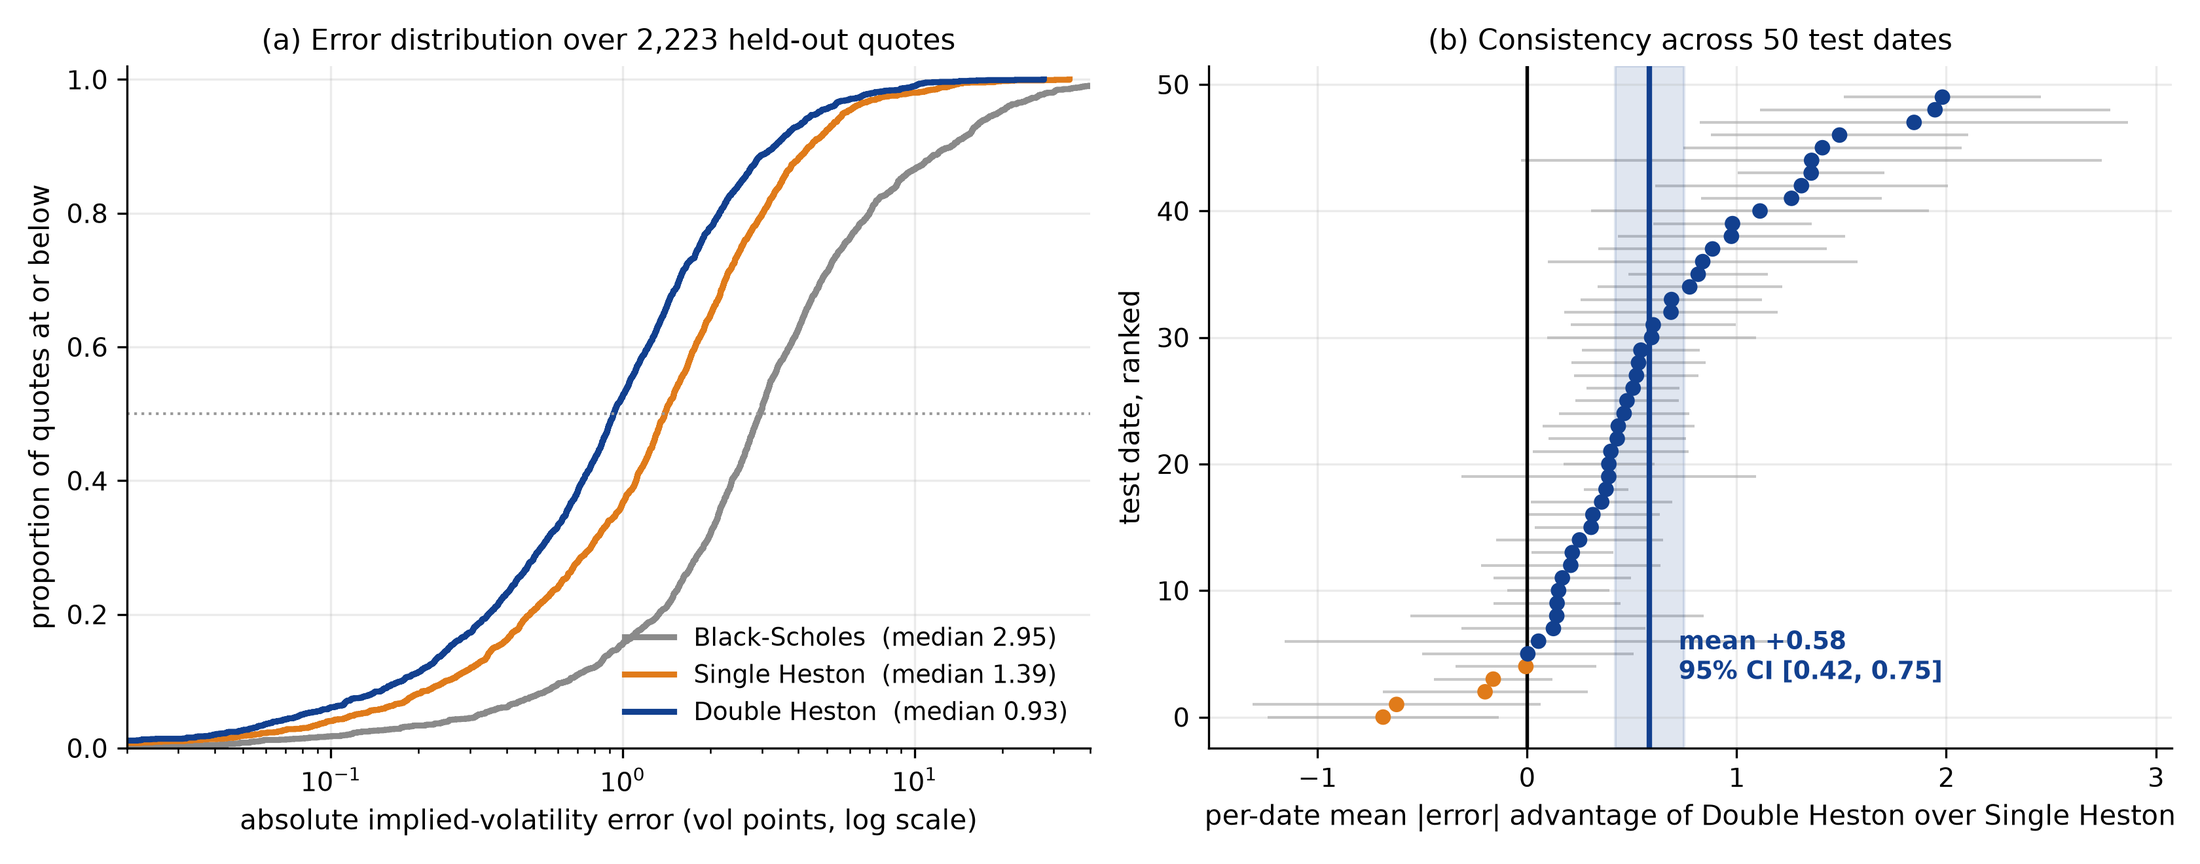
\includegraphics[width=\textwidth]{fig3_statistical_evidence.png}
\caption{Descriptive view of Bitcoin held-out errors, pooled over all 50 test
dates (2{,}223 quotes). (a)~Empirical cumulative distribution of absolute
implied-volatility error; Double Heston lies left of Single Heston at every
quantile. (b)~Per-date mean paired advantage of Double Heston over Single
Heston, ranked, with 95\% intervals; the shaded band is the cluster-bootstrap
interval for the overall mean. These are descriptive statistics pooled across
regimes and are not the pre-specified endpoint of Table~\ref{tab:results}.}
\label{fig:stats}
\end{figure}

\subsection{The Pattern Behind the Split}
\label{sec:split}

The division is not random with respect to market structure.
Table~\ref{tab:markets} reports the median number of distinct expiries quoted
per evaluation date: Bitcoin quotes seven and Ether six, while Solana, XRP and
Hyperliquid quote about four. The two markets in which the second variance
factor pays are exactly the two that quote the most maturities.

This is what identifiability predicts. Two mean-reversion speeds can be
separated only if the data contain maturities at which their effects differ.
With four expiries, often with two or three clustered inside a month, a fast
and a slow factor produce nearly the same fitted surface, and the second factor
adds parameters without adding explanatory power. With six or seven expiries
spanning days to several months, the two time scales leave distinguishable
fingerprints and the extra factor earns its place.

The contrast between the two held-out designs sharpens this reading rather
than undermining it. Under Design~A every maturity
is still present in the calibration set and a model has only to interpolate
across strikes; no separation of time scales is required, and the extra
flexibility of a second factor helps almost everywhere, clearing the criterion
in seven of nine cells including Solana shock, XRP shock and Hyperliquid.
Under Design~B an entire maturity is removed, interpolation across the term
structure becomes necessary, and the same model clears the criterion in only
the four Bitcoin and Ether cells. The second factor is therefore not useless
in the thin markets: it fits them perfectly well when it does not have to
place them in maturity. What the thin surfaces cannot support is the
\emph{identification} of two distinct speeds, and that is precisely the
capability Design~B tests and Design~A does not. We regard the divergence
between the two designs as the clearest single piece of evidence for the
mechanism we propose.

\subsection{Illustration on a Single Surface}

Figure~\ref{fig:cvss} shows one Bitcoin surface with all three models
calibrated to that date. Single Heston lies above the quotes and
Black--Scholes below them, while Double Heston passes through them; within the
plotted moneyness window the Double-Heston price error is 4.7 times smaller
than the better baseline. Panel~(b) shows the step in the Black--Scholes curve
where it switches between expiry knots, a structural consequence of granting it
one volatility per expiry. Two caveats apply: the expiry shown is a
calibration expiry rather than a held-out one, so all three models are
in-sample on it, and the ratio is computed over the seven quotes inside the
window rather than all twenty. A single surface is an illustration, not
evidence; the evidence is the pre-specified aggregate in
Table~\ref{tab:results}.

\begin{figure}[htbp]
\centering
\begin{minipage}[b]{0.495\textwidth}\centering
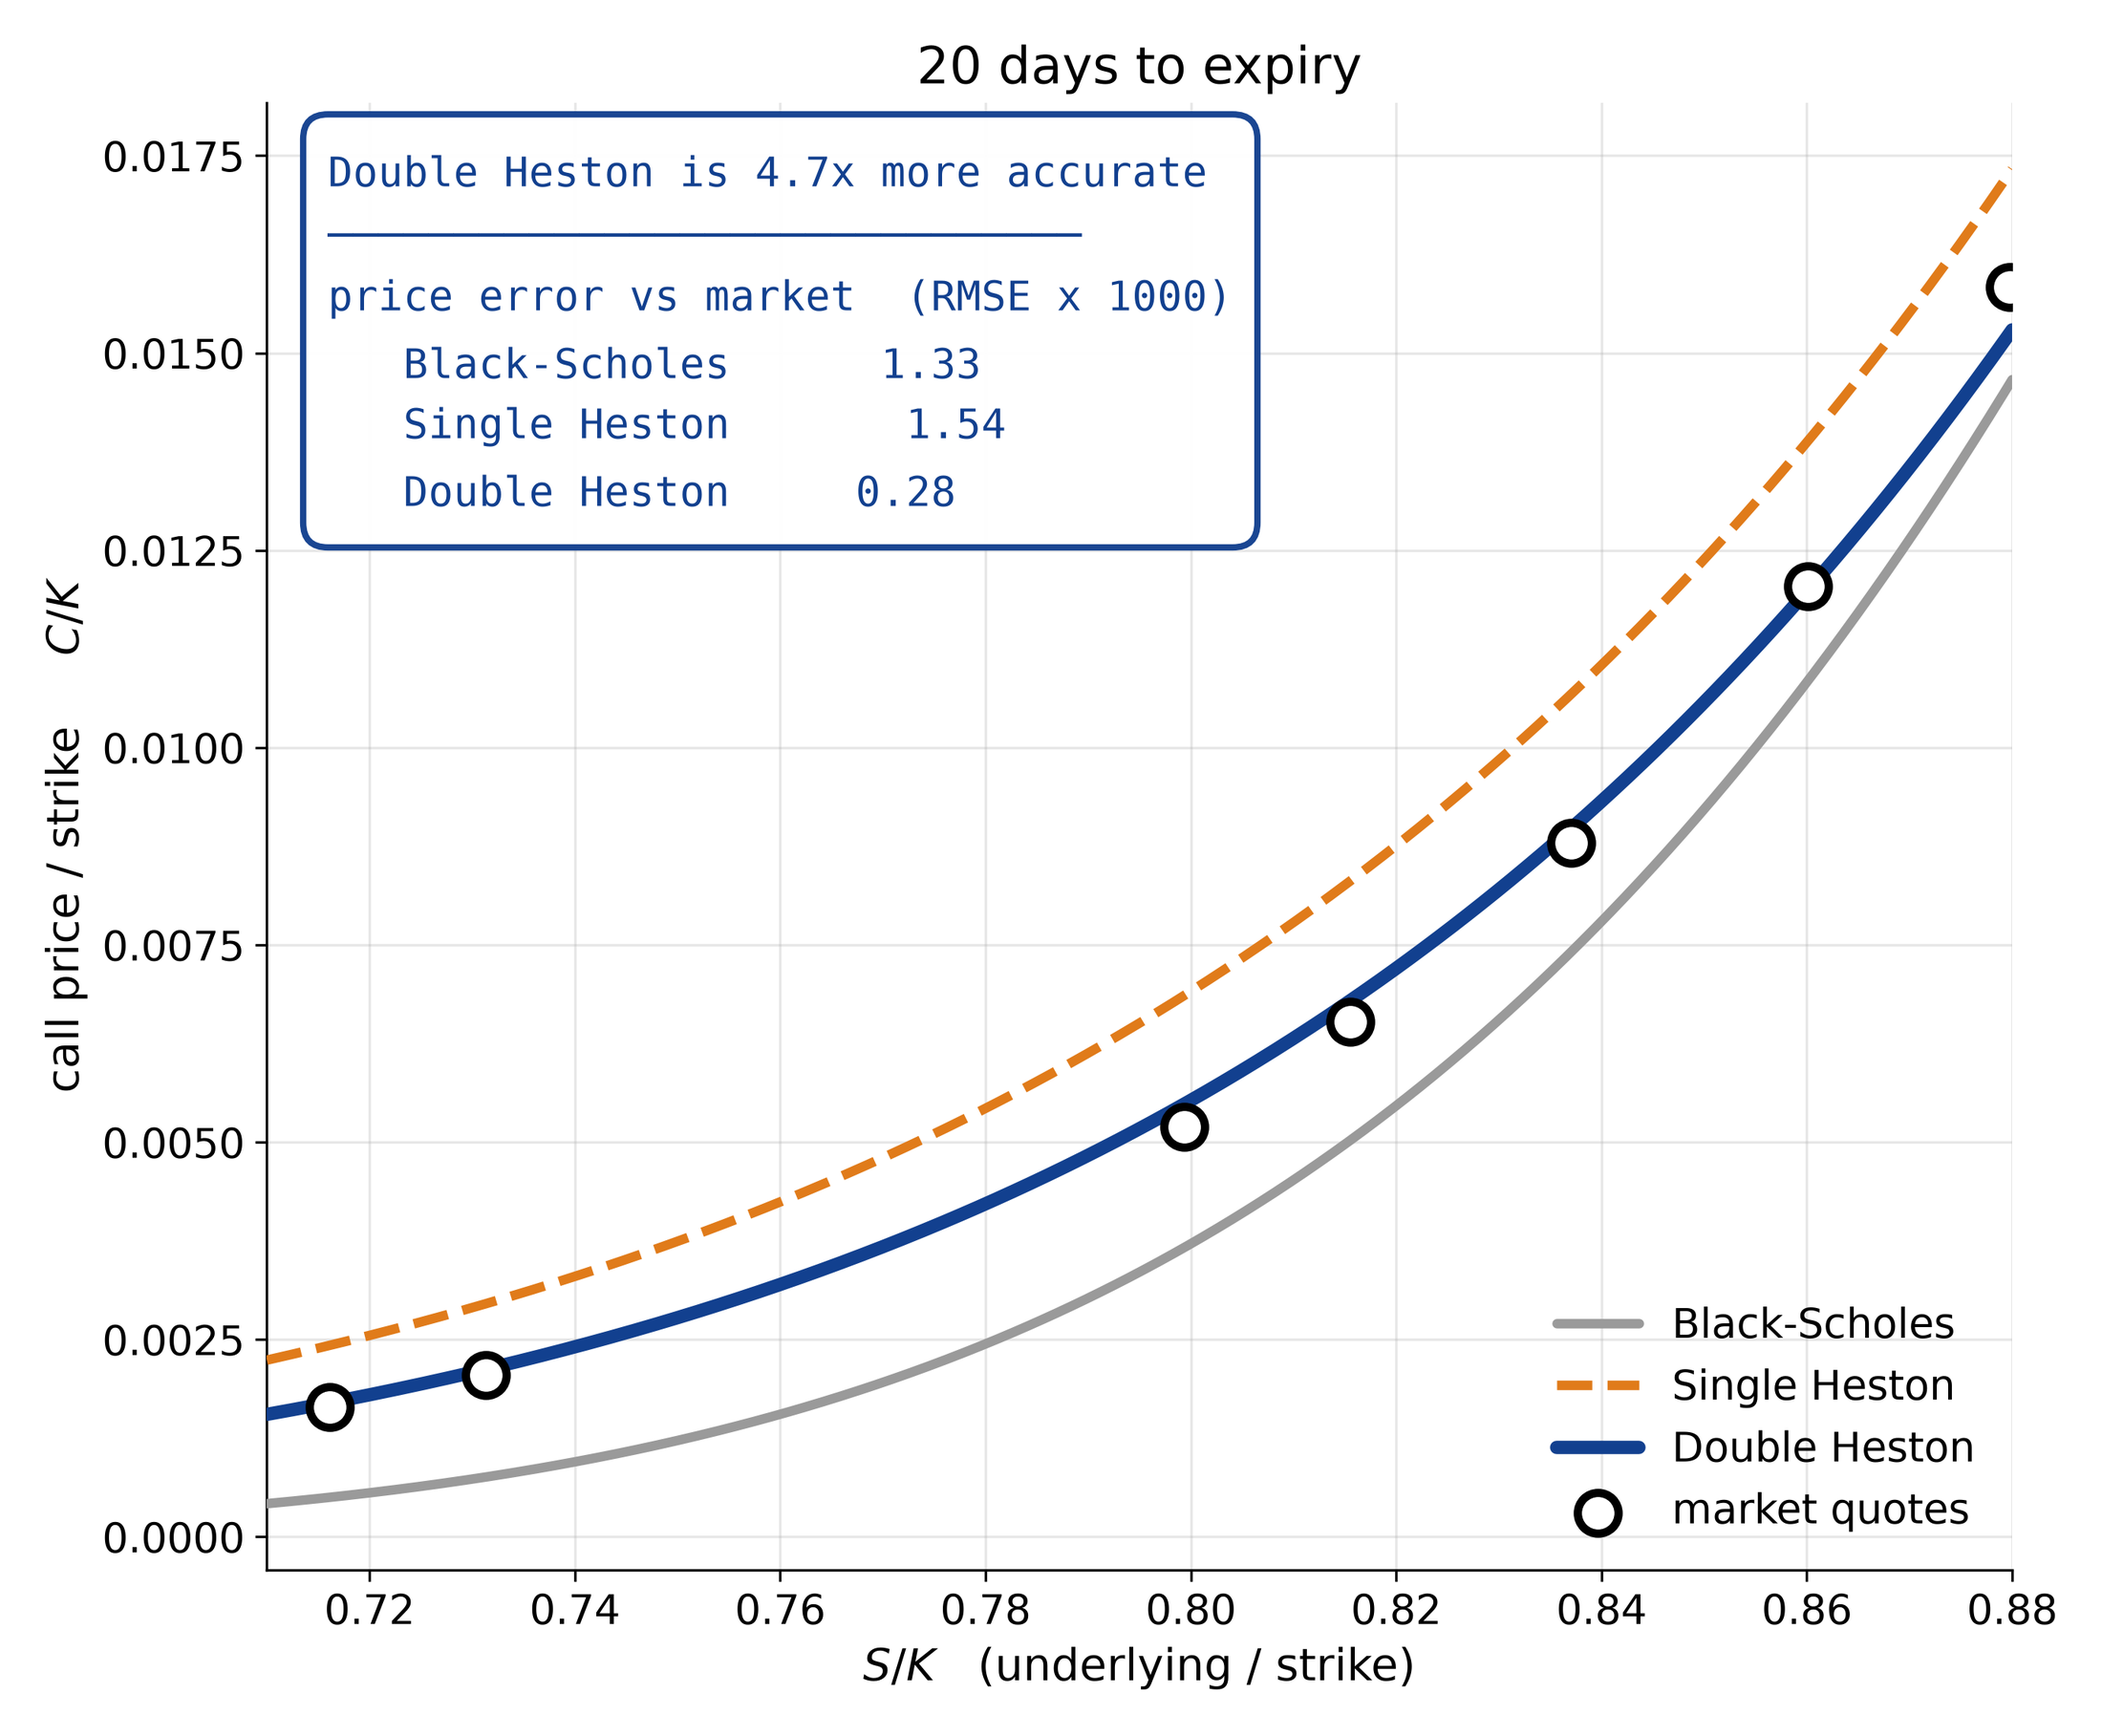
\includegraphics[width=\linewidth]{fig1_C_vs_S.png}\\[0.2ex]
{\footnotesize (a) against underlying price}
\end{minipage}\hfill
\begin{minipage}[b]{0.495\textwidth}\centering
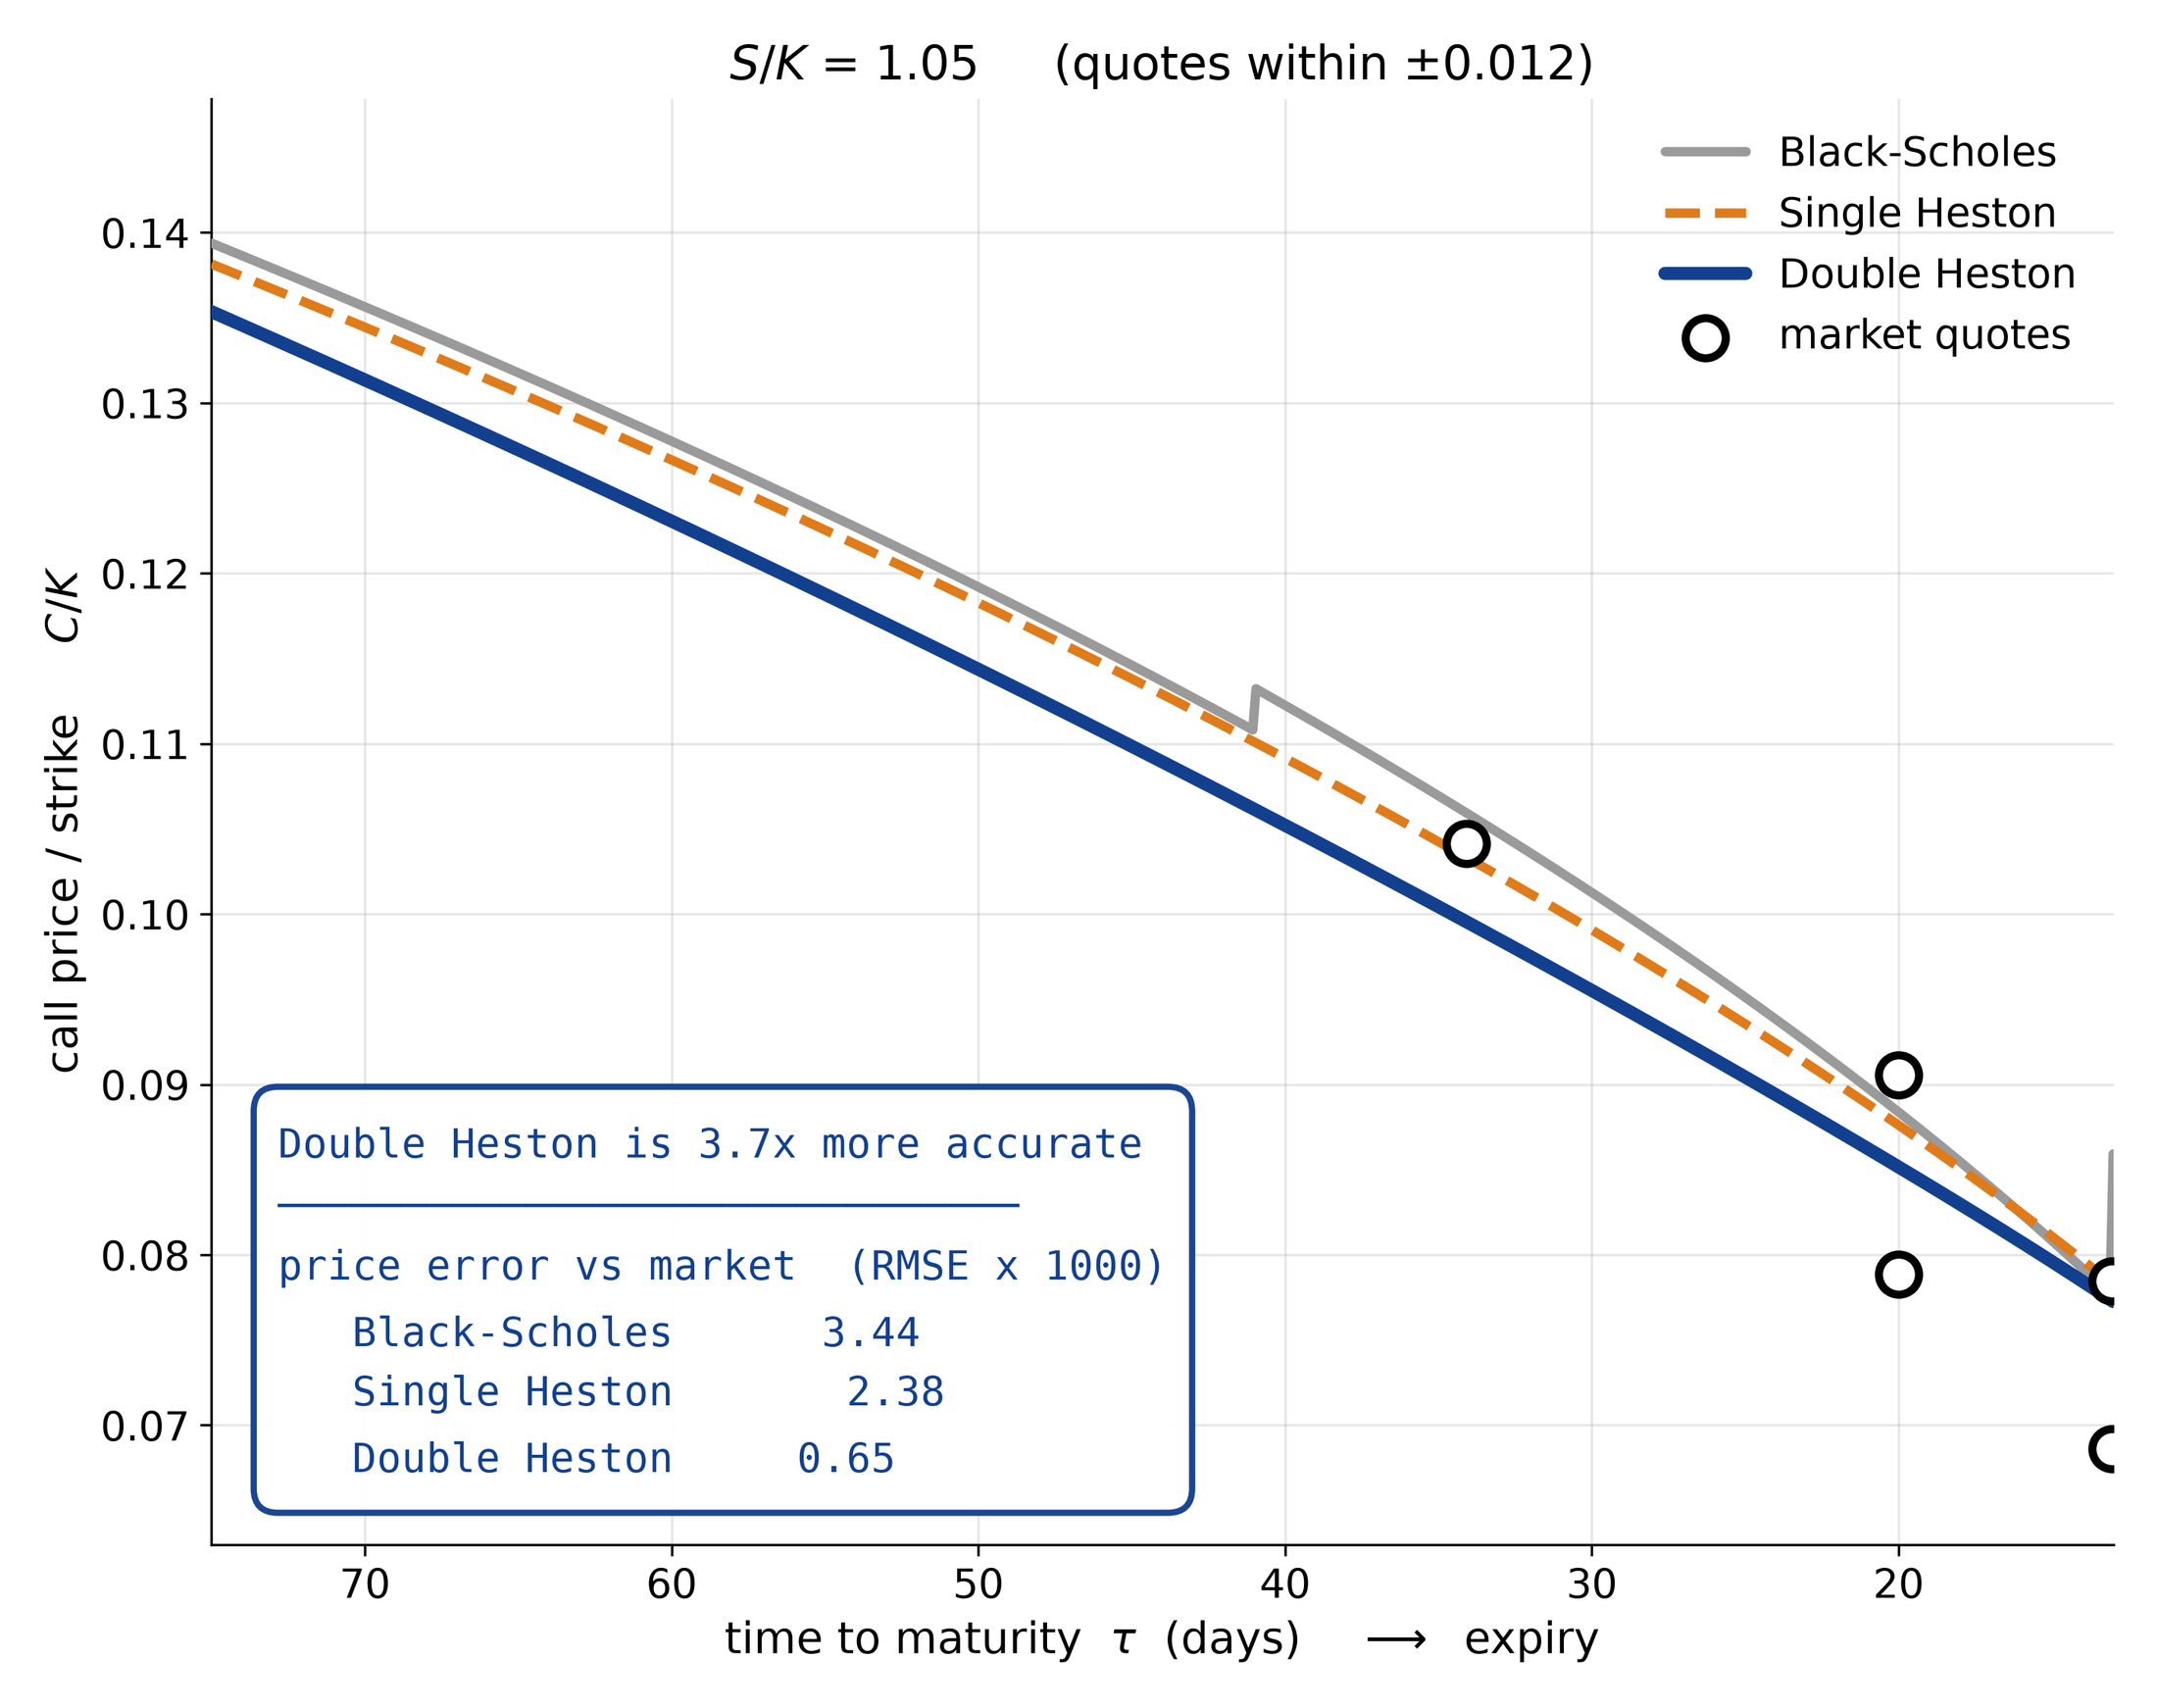
\includegraphics[width=\linewidth]{fig2_C_vs_tau.png}\\[0.2ex]
{\footnotesize (b) against time to maturity}
\end{minipage}
\caption{One Bitcoin surface, 27~July 2024, all three models calibrated to that
date. (a)~Call price against underlying price for the 20-day expiry. That
expiry is ranked second of the eight quoted that day and so belongs to the
Design~B \emph{calibration} set: the comparison is in-sample, shown only to
illustrate the shape of the three fitted surfaces, and the error figures
printed in the panel are computed over the seven quotes inside the plotted
moneyness window, not over all twenty in the expiry. (b)~Call price against
time to maturity at fixed moneyness; maturity decreases left to right, so each
curve decays towards its payoff at expiry, and the step in the Black--Scholes
curve marks a switch between expiry knots. The held-out evidence is
Table~\ref{tab:results}.}
\label{fig:cvss}
\end{figure}


% =====================================================================
\FloatBarrier

Because a single surface can be chosen favourably, Figure~\ref{fig:range}
shows three surfaces side by side: the date on which Double Heston holds its
largest advantage, the date at the median advantage, and the date on which
Single Heston wins by the largest margin. On that last date the one-factor
model is the more accurate of the two. Reporting the unfavourable end of the
range is the reason the aggregate in Table~\ref{tab:results} should be read as
the result, and any single surface only as an illustration.

\begin{figure}[htbp]
\centering
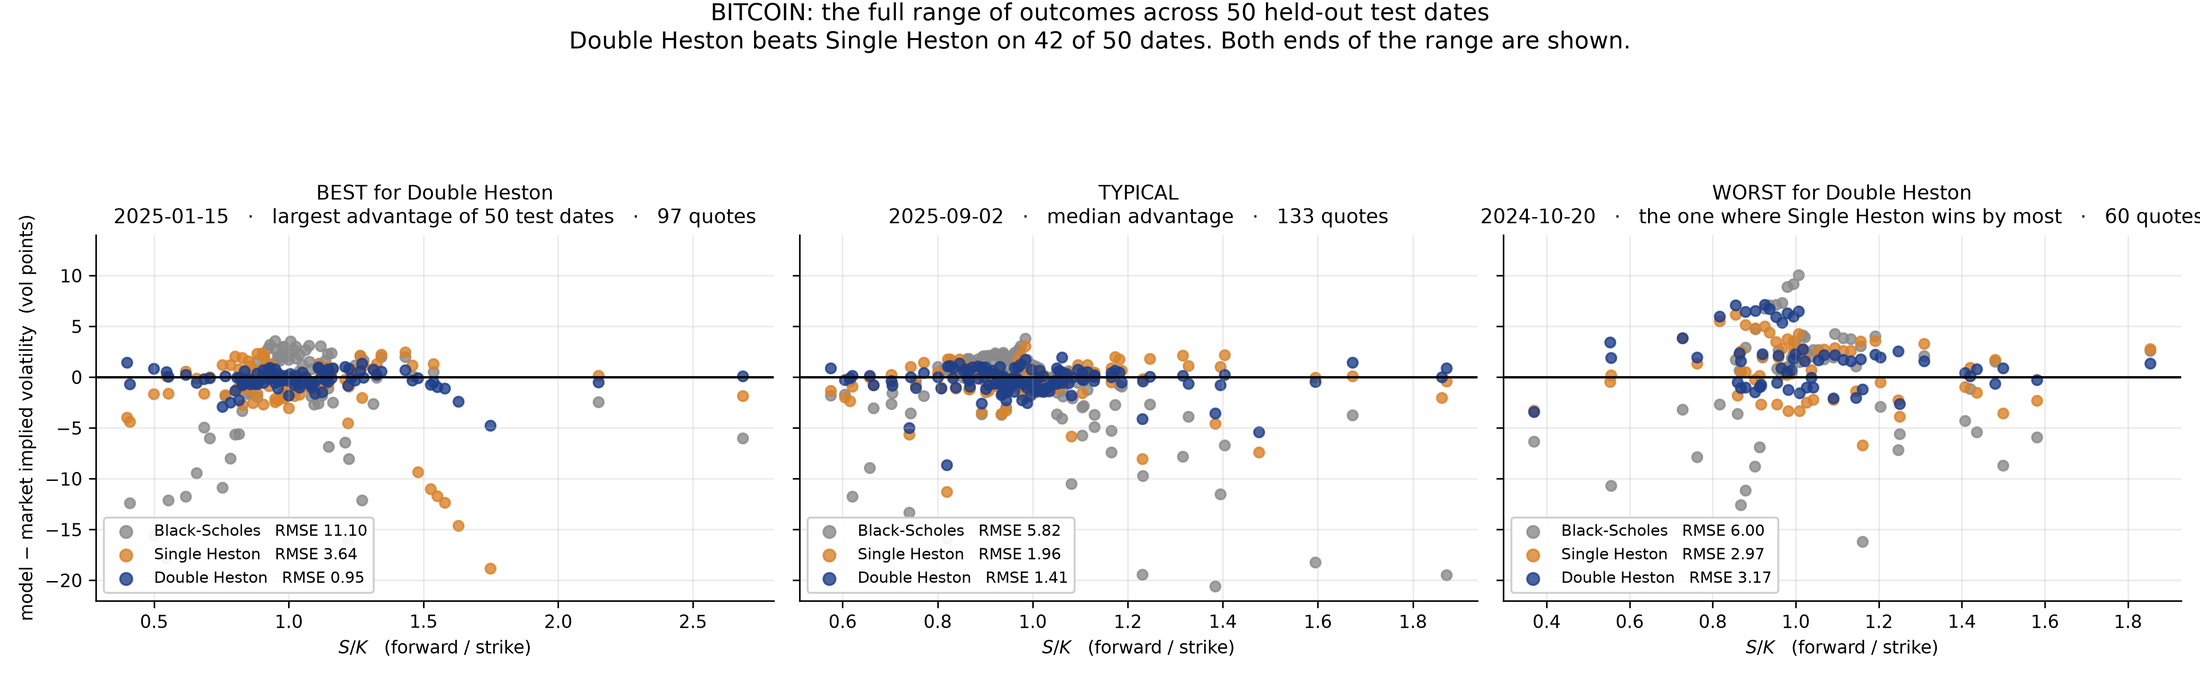
\includegraphics[width=\textwidth]{fig4_range_of_outcomes.png}
\caption{Range of single-date outcomes on Bitcoin, showing model minus market
implied volatility against moneyness. Left: the test date on which Double
Heston holds its largest advantage. Centre: the date at the median advantage.
Right: the date on which Single Heston wins by the largest margin. Both ends of
the range are shown so that the illustration in Figs.~\ref{fig:cvss}
and~\ref{fig:cvss} is not mistaken for a typical case.}
\label{fig:range}
\end{figure}

\section{Discussion}

The headline result of most model-comparison papers is that the richer model
wins. Ours is that the richer model wins \emph{when the data can identify it},
and that this condition fails in three of the five markets examined.

This reframing matters for three reasons. It is actionable: a practitioner
can inspect the expiry count of the surface they actually trade rather than
rely on a result obtained on a richer market. It explains conflicting results
in the literature without invoking implementation differences, since studies
on major equity indices with dozens of listed expiries should find a
two-factor advantage and studies on thin surfaces should not. And it suggests
the useful question is not which model is better but how much structure a
given surface can support: a model that cannot be identified is not a better
model hidden by noise, it is an over-specified model whose extra parameters
absorb noise.

Solana calm dates, where the point estimate favours the one-factor model, are
consistent with this reading. Over-specification need not merely fail to help;
it can hurt, when the extra freedom fits features of the calibration set that
do not recur out of sample.

% =====================================================================
\section{Limitations}
\label{sec:limitations}

One feature of the sampling deserves explicit statement because it bears
directly on our central variable. A date enters the sample only if it quotes a
minimum number of distinct expiries, and that minimum was five for Bitcoin and
Ether but four for Solana, XRP and Hyperliquid, because a common threshold of
five would have excluded most of the thinner markets entirely. The
expiry-count contrast in Table~\ref{tab:markets} is therefore measured under
inclusion rules that differ across markets, and part of the gap is induced by
those rules rather than observed freely. The direction is conservative --- a
common threshold of five would have removed the thin markets' least rich
surfaces and \emph{raised} their median expiry count --- but we cannot claim
the grouping is independent of the filter, and a replication should fix one
threshold throughout.

The study covers a single venue (Deribit). Crypto surfaces are steeper and
thinner than equity surfaces, so the threshold we observe, roughly six
expiries per day, should not be transferred to other asset classes without
re-testing; the mechanism should transfer, the number need not. Expiry count
is also not the only difference between these markets: Bitcoin and Ether are
older, more liquid and longer-listed, and with five markets we cannot fully
separate maturity coverage from liquidity. Expiry count is the variable
identifiability theory singles out and it orders the results without
exception, but a larger cross-section would be needed to isolate it.

Hyperliquid has the shortest history of the five markets: its 55 evaluation
dates fall inside one short listing window and are clustered by ISO week rather
than by volatility episode, so its 13 clusters are less independent than the
episode clusters used elsewhere. Our calibration
bounds bind in a large share of fits: the volatility-of-variance upper bound is
reached in 63 of 132 one-factor fits (48\%), and in 80 of 132 (61\%, slow
factor) and 76 of 132 (58\%, fast factor) two-factor fits. Relaxing those bounds after seeing the results is not
permitted under our own protocol, so we record it as the leading candidate
improvement for a future, independently pre-registered experiment. Finally, we
measure pricing accuracy on held-out quotes from the same day; forecasting,
hedging performance and economic value are separate questions.

% =====================================================================
\section{Conclusion}

We compared Black--Scholes, Heston and Double Heston on 16,186 option
quotes from five cryptocurrency markets, 5,214 of them held out under the
primary design, under a protocol fixed and hashed before any option data was
seen. The two-factor model beat the constant-volatility
baseline everywhere, cutting median held-out implied-volatility error on
Bitcoin shock dates from 8.13 to 1.86 volatility points. Against the one-factor
model it won decisively on Bitcoin and Ether and failed to win on Solana, XRP
and Hyperliquid, with one market in which the point estimate favoured the
simpler model though our two-part criterion was not met in that direction.

The two markets in which the second variance factor paid are the two that quote
six to seven expiries per day; the three in which it did not quote about four.
We read this as an identifiability boundary rather than a property of the
model. The practical implication is that the choice between one and two
variance factors should be made by inspecting the surface, not only the model.
The methodological implication is that pre-specifying the selection rule and
requiring two independent significance criteria changed our conclusions: two
results that a single test would have reported as wins did not survive both.

% =====================================================================
\begin{thebibliography}{99}

\bibitem{black1973}
Black, F., Scholes, M.: The pricing of options and corporate liabilities.
J. Polit. Econ. \textbf{81}(3), 637--654 (1973)

\bibitem{merton1973}
Merton, R.C.: Theory of rational option pricing. Bell J. Econ. Manag. Sci.
\textbf{4}(1), 141--183 (1973)

\bibitem{black1976}
Black, F.: The pricing of commodity contracts. J. Financ. Econ.
\textbf{3}(1--2), 167--179 (1976)

\bibitem{gatheral2006}
Gatheral, J.: The Volatility Surface: A Practitioner's Guide. Wiley, Hoboken
(2006)

\bibitem{heston1993}
Heston, S.L.: A closed-form solution for options with stochastic volatility
with applications to bond and currency options. Rev. Financ. Stud.
\textbf{6}(2), 327--343 (1993)

\bibitem{bakshi1997}
Bakshi, G., Cao, C., Chen, Z.: Empirical performance of alternative option
pricing models. J. Finance \textbf{52}(5), 2003--2049 (1997)

\bibitem{bates2000}
Bates, D.S.: Post-'87 crash fears in the S\&P 500 futures option market.
J. Econom. \textbf{94}(1--2), 181--238 (2000)

\bibitem{duffie2000}
Duffie, D., Pan, J., Singleton, K.: Transform analysis and asset pricing for
affine jump-diffusions. Econometrica \textbf{68}(6), 1343--1376 (2000)

\bibitem{chj2009}
Christoffersen, P., Heston, S., Jacobs, K.: The shape and term structure of the
index option smirk: why multifactor stochastic volatility models work so well.
Manag. Sci. \textbf{55}(12), 1914--1932 (2009)

\bibitem{carr1999}
Carr, P., Madan, D.B.: Option valuation using the fast Fourier transform.
J. Comput. Finance \textbf{2}(4), 61--73 (1999)

\bibitem{fang2008}
Fang, F., Oosterlee, C.W.: A novel pricing method for European options based on
Fourier-cosine series expansions. SIAM J. Sci. Comput. \textbf{31}(2),
826--848 (2008)

\bibitem{lord2010}
Lord, R., Kahl, C.: Complex logarithms in Heston-like models. Math. Finance
\textbf{20}(4), 671--694 (2010)

\bibitem{cui2017}
Cui, Y., del Ba\~{n}o Rollin, S., Germano, G.: Full and fast calibration of the
Heston stochastic volatility model. Eur. J. Oper. Res. \textbf{263}(2),
625--638 (2017)

\bibitem{feller1951}
Feller, W.: Two singular diffusion problems. Ann. Math. \textbf{54}(1),
173--182 (1951)

\bibitem{madan2019}
Madan, D.B., Reyners, S., Schoutens, W.: Advanced model calibration on bitcoin
options. Digit. Finance \textbf{1}, 117--137 (2019)

\bibitem{hou2020}
Hou, A.J., Wang, W., Chen, C.Y.H., H\"{a}rdle, W.K.: Pricing cryptocurrency
options. J. Financ. Econom. \textbf{18}(2), 250--279 (2020)

\bibitem{alexander2021}
Alexander, C., Imeraj, A.: The Bitcoin VIX and its variance risk premium.
J. Altern. Invest. \textbf{23}(4), 84--109 (2021)

\bibitem{alexander2023}
Alexander, C., Imeraj, A.: Delta hedging bitcoin options with a smile.
Quant. Finance \textbf{23}(5), 799--817 (2023)

\bibitem{wilcoxon1945}
Wilcoxon, F.: Individual comparisons by ranking methods. Biom. Bull.
\textbf{1}(6), 80--83 (1945)

\bibitem{efron1979}
Efron, B.: Bootstrap methods: another look at the jackknife. Ann. Stat.
\textbf{7}(1), 1--26 (1979)

\bibitem{cameron2008}
Cameron, A.C., Gelbach, J.B., Miller, D.L.: Bootstrap-based improvements for
inference with clustered errors. Rev. Econ. Stat. \textbf{90}(3), 414--427
(2008)

\bibitem{nosek2018}
Nosek, B.A., Ebersole, C.R., DeHaven, A.C., Mellor, D.T.: The preregistration
revolution. Proc. Natl. Acad. Sci. \textbf{115}(11), 2600--2606 (2018)

\end{thebibliography}

\end{document}
